 \chapter{Stato dell'arte e strumenti}

% **************************** Define Graphics Path **************************
\ifpdf
    \graphicspath{{Chapter4/Figs/Raster/}{Chapter4/Figs/PDF/}{Chapter4/Figs/}}
\else
    \graphicspath{{Chapter4/Figs/Vector/}{Chapter4/Figs/}}
\fi

\section{Stato dell'arte}
La possibilità di impiegare i droni come relays in una FANET li rende una possibile soluzione in situazioni dove gruppi di nodi a terra rimangono isolati dal resto della rete. \\
In letteratura sono stati proposti vari algoritmi e tecniche per risolvere il posizionamento ottimo di droni in una rete ad-hoc. \\
In \cite{Sahingoz2014, 6477822} gli autori descrivono il problema da un punto di vista del networking, affermando che una delle principali key enabling technologies per lo sviluppo futuro delle FANET sia la progettazione di nuovi protocolli di rete e l'adattamento di quelli attuali, dato che le FANET introducono nuove sfide e requisiti. \\
In \cite{1023918} e \cite{Burdakov2010} gli autori propongono un modello MILP centralizzato per coordinare il volo di un gruppo di droni e evitare le collisioni con eventuali ostacoli. \\
In \cite{6564778}, il problema di posizionare i droni in una rete hub-and-spoke per interconnettere un insieme di client viene formulato come problema MILP, e viene fornito un approccio di Quadratic Integer Programming per determinare la topologia a minimo costo della rete.
Gli autori concludono affermando che, seppure un approccio quadratico riduca notevolmente il numero di vincoli e abbia performance migliori, rispetto la controparte lineare, la ricerca di un modello lineare, qualora possibile, sarebbe sempre da preferire grazie alle tecniche di risoluzione di alta qualità disponibili.\\
In \cite{4455114} il modello proposto si focalizza sull'impiego un drone per migliorare la connettività della rete ad-hoc sottostante, ottimizzando i flussi di traffico con un modello multi-commodity flow, ma considera la presenza di un singolo drone e assume che gli utenti sottostanti siano già tra loro interconnessi, oltre a non considerare il problema dell'interferenza. \\
Per la risoluzione di questo problema sono stati proposti anche approcci distribuiti, come in \cite{Correll09ad-hocwireless}, dove le decisioni sul posizionamento e lo spostamento sono delegate ai droni, che sono in grado di apprendere informazioni sullo stato della rete e sulle loro posizioni reciproche e agire di conseguenza, e in \cite{6162393}, in cui gli UAV usano sensori (come il GPS) o parametri di rete (come il Received Signal Strength Indicator, o RSSI) per posizionarsi nello spazio e ottimizzare la comunicazione con i nodi a terra. \\
Un altro approccio ampiamente usato è quello delle metaeuristiche: in \cite{5983050} vengono proposti e confrontati due algoritmi, basati su Hill Climbing e Tabu Search, che valutano le posizioni migliori in cui disporre dei nodi di supporto che permettano di riconnettere sezioni della rete originale rimasti isolati, in \cite{1495151} gli autori realizzano un algoritmo dinamico per minimizzare il numero di droni, prendendo in considerazione il problema del movimento casuale dei client e dei protocolli di routing necessari ma senza analizzare il problema dell'interferenza, mentre in \cite{Rohde20131893} si impiega un algoritmo genetico per posizionare i nodi relay in modo da massimizzare il throughput della rete e consentire il self-healing dei link che diventano offline. \\     
Per quanto riguarda la gestione dell'interferenza, è generalmente molto complesso predirla in maniera statica, a causa della dinamicità dell'ambiente in cui la rete si trova e dei fattori che concorrono a causarla. Di  conseguenza, generalmente si cerca di valutarla in tempo reale monitorando determinati parametri di qualità della rete \cite{Halperin:2010:PPD:1851275.1851203,6151307} e di prevenirla attraverso opportune scelte di design in fase di progettazione, pe resempio tramite channel allocation \cite{7383864}. \\

\section{Interferenza radio}
Nelle comunicazioni wireless la minimizzazione dell'interferenza è un problema primario, dato che al suo crescere aumenta il rischio di collisione tra pacchetti e la conseguente necessità di ritrasmissione, riducendo le performance globali della rete. \\
Poichè nelle reti wireless il mezzo trasmissivo non è un canale fisico, abbiamo dovuto traslare il concetto di capacità massima dal punto di vista del canale a quello del nodo. Questo significa che che ogni nodo è caratterizzato da una capacità trasmissiva massima ottimale $U_{TX}$ e da una capacità di ricezione massima ottimale $U_{RX}$. Questi due valori rappresentano il numero massimo di pacchetti (visti come parte di un flusso) che un nodo può inviare o ricevere in un dato istante di tempo in un ambient eprivo di interferenza. \\
Il modello di interferenza che descriveremo è basato sul punto di vista del ricevente \cite{Rickenbach05arobust}, cioè ogni nodo subisce interferenza da qualunque nodo stia trasmettendo all'interno del suo range. Considereremo l'interferenza dal punto di vista del physical layer. \\
L'obbiettivo principale nella modellizzazione dell'interferenza è stato quello di mantenerla al di fuori del modello MILP, cosicchè fosse possibile applicare un qualunque modello, di complessità arbitraria, senza preoccuparsi dei vincoli di linearità.
Abbiamo perciò definito un modello statico e locale di interferenza basato sulla distribuzione spaziale dei nodi e sul loro range trasmissivo. Tale modello calcola la riduzione di capacità dei nodi e la fornisce in output sotto forma di fattore di sconto, che può essere impiegato come coefficiente nel modello MILP, mantenendo la linearità del modello.

\subsection{Modello di interferenza}
Dato che l'interferenza radio dipende da una pluralità di fattori, generalmente molto difficili da determinare a priori e senza dati sperimentali, abbiamo dovuto imporre una forte semplificazione al modello, ovvero che l'interferenza venga valutata tra ogni coppia di nodi mittente-destinatario assumendo che nessun'altra trasmissione stia avvenendo entro il loro range. Questo comporta la riduzione delle sorgenti di interferenza alle sole caratteristiche dell'ambiente e al path loss \cite{Killat:2009:EMP:1554307.1554311}, che possono essere determinati staticamente tramite approssimazioni e modelli empirici. \\
L'interferenza totale che un nodo subisce sarà quindi proporzionale al numero di nodi che trasmettono all'interno del suo range di comunicazione \cite{moaveni2005low}, e verrà scontata dalla capacità ottimale di ricezione $U_{RX}$. \\
Nel caso di elevato livello di interferenza (ad esempio se due droni sono molto vicini tra loro), limitato superiormente al valore $S_{max}$, assumiamo che una minima frazione della capacità $U_{RX}$ sia sempre garantita. Questo livello minimo di capacità, per ogni nodo, è un parametro del modello e corrisponde all'efficienza minima dei protocolli di reti wireless classici \cite{tanenbaum2003computer}. \\
Ogni nodo è caratterizzato da un'area di trasmissione circolare con raggio $R$, al cui interno gli altri nodi possono riceverne i dati inviati. Questa area trasmissiva coincide con l'area totale di interferenza, perciò se la distanza tra due nodi $i$ e $j$ è maggiore di $R$, le trasmissioni di $i$ non interferiranno con $j$ e viceversa.  \\
Definiamo con $A_{ij}$ il coefficiente di interferenza, inteso come riduzione di capacità, che il nodo $j$ subisce a causa della vicinanza del nodo $i$. Si noti che, in questo modello, $A_{ij} = A_{ji}$.
In base alla distanza reciproca fra due nodi, il fattore di interferenza viene valutato in due modi differenti. \\
Per ciascun nodo, definiamo una seconda area circolare di raggio $R_\epsilon$ ($R_\epsilon << R$), detta Area Critica, al cui interno l'interferenza causata da un eventuale nodo è massima, e la corona circolare identificata dalla differenza delle aree trasmissiva e critica, come si può vedere in \figurename\ \ref{fig:noderange}. \\

\begin{wrapfigure}{R}{0.5\textwidth}
	\begin{center}
		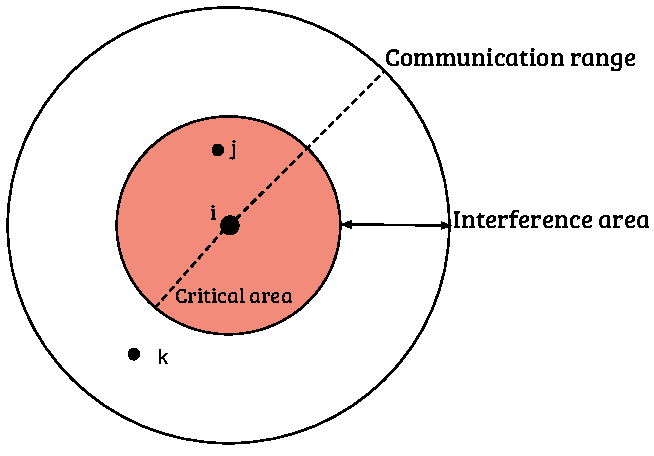
\includegraphics[scale=0.75]{noderange}
	\end{center}
	\caption{Schema del range di comunicazione di un nodo\label{fig:noderange}}
\end{wrapfigure}

L'area critica è la zona in cui ogni nodo è più sensibile all'interferenza. Per questo motivo, dati due nodi $i$ e $j$ e la funzione $d(x,y)$ che ne calcola la distanza geometrica, se $d(i,j) < R_\epsilon $ i due nodi si interferiranno a vicenda in maniera massima, quindi $A_{ij} = S_{max}$.
La presenza di molteplici nodi in questa zona non annullerà comunque la capacità minima garantita. \\
Se invece i nodi più vicini ad $i$ si trovano nella corona circolare, allora l'interferenza totale subita da $i$ può essere valutata simulando un Radio Propagation Model, e sarà proporzionale al numero di questi nodi e alla loro distanza da $i$, pur senza superare il livello massimo di interferenza $S_{max}$ consentito dal modello. 


\subsection{ns-2 Radio Propagation Model}
I coefficienti dell'area di interferenza $A_{ij}$ vengono valutati staticamente utilizzando un Radio Propagation Model \cite{seybold2005introduction}, ovvero un modello matematico empirico che descrive e formalizza la propagazione delle onde radio in funzione della frequenza, della distanza, dell'ambiente circostante e di altri parametri. \\
Lo scopo principale di questi modelli è determinare l'attenuazione che il segnale radio (path loss) subisce nel tragitto fra la trasmittente e il ricevente, in quanto essa è il fattore principale che permette di caratterizzare come l'onda si propaga. Lo scopo secondario è quello di stimare l'area di comunicazione di una trasmittente.\\
Poiché ogni link wireless è soggetto a differenti fenomeni di interferenza (ostacoli, condizioni ambientali, terreni), è chiaramente impossibile modellare e prevedere in maniera esatta il path loss per ciascun sistema. Di conseguenza sono nati numerosi modelli, ciascuno specializzato per determinate condizioni e ambienti. \\
I radio propagation models sono totalmente empirici, perché sviluppati su ampi campioni di dati raccolti in specifici scenari, quindi non sono in grado di predire il path loss esatto, ma il suo comportamento generale in quel determinato set di condizioni.  \\
Il modello che abbiamo deciso di impiegare è lo Shadowing Model implementato dal simulatore di rete ns-2 \cite{nsMan}, in quanto rappresenta un buon compromesso tra accuratezza, generalità e semplicità di implementazione. \\
Nello shadowing model il range di comunicazione di ogni nodo è più realistico, in quanto non è un cerchio ideale, ma presenta frastagliature e irregolarità crescenti man mano che ci si allontana dal centro (\figurename\ \ref{fig:shadowing}), per simulare gli effetti del multipath propagation. \\

\begin{wrapfigure}{R}{0.5\textwidth}
	\begin{center}
		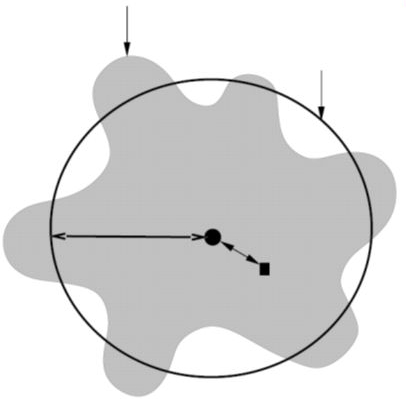
\includegraphics[scale=0.60]{shadowing}
	\end{center}
	\caption{Range di comunicazione nello Shadowing Model\label{fig:shadowing}}
\end{wrapfigure}

Tale fenomeno, presente in ogni comunicazione radio, è causato dalla propagazione in più direzioni di un segnale trasmesso da un'antenna: ciascuna copia del segnale compie percorsi diversi e incontra diversi ostacoli e superfici (acqua, terreno, edifici, montagne, veicoli, etc.), subendo distorsioni prima di sommarsi al segnale originale, introducendo interferenze \cite{umar2004mobile}. \\
La scelta di questo modello ha come conseguenza che vi è una probabilità non nulla che i messaggi trasmessi entro il range del destinatario non vengano ricevuti. Questa probabilità cresce al crescere della distanza dal nodo ricevente. \\
Vale la pena far notare che la forma più realistica del range di comunicazione non interferisce con le precedenti assunzioni di un'area trasmissiva circolare perfetta, impiegata all'interno del modello MILP.\\
Nel modello di interferenza di ns-2, ogni nodo ha un parametro $rxThresh$ che rappresenta la soglia di ricezione del segnale: quando un pacchetto viene ricevuto, se ne testa la potenza di segnale ($P_r$) con $rxThresh$, e se $ P_r \geq rxThresh$ il pacchetto viene considerato ricevuto correttamente. \\
Per semplificare il calcolo, assumeremo che la variazione della potenza di segnale tra pacchetti dello stesso flusso, valutata dal modello, sia trascurabile. \\
Successivamente, il valore $P_r$ calcolato dal modello di interferenza deve essere tradotto in una percentuale di riduzione della capacità, per poter essere impiegato nel MILP. Questa procedura viene eseguita come pre-elaborazione nel seguente modo:
\begin{enumerate}  
	\item Si calcola $P_r$ per ogni coppia ($i$,$j$) di nodi trasmittente-ricevente un numero significativamente alto di volte, per ottenere la frequenza relativa $f_{flow}^{i,j}$ con cui $P_r$ supera il valore $rxThresh$. Questo valore rappresenta una stima della probabilità che il flusso di traffico trasmesso sia interamente ricevuto con successo;
	\item Si mappa il valore $f_{flow}^{i,j}$ ottenuto su una scala percentuale di interferenza che va da $0$ (nessuna interferenza) a $S_{max}$ (massima interferenza ammessa dal modello);
	\item Il valore risultante costituisce il coefficiente $A_{ij}$ e può essere impiegato nel modello MILP come valore percentuale di riduzione della capacità totale del nodo $i$ a causa della presenza del nodo $j$.
\end{enumerate}







